\documentclass[utf8]{beamer}
\usepackage[UTF8,noindent]{ctexcap}
\usepackage{amsmath}

\title{Hanakiko的日常}
\subtitle{题解与讲评}
\institute{南宁市第三中学}
\author{Sweetlemon}
\date{\today}
\definecolor{miku}{HTML}{39c5bb}
\definecolor{tianyi}{HTML}{66ccff}
\definecolor{admin}{HTML}{8e44ad}
\definecolor{tle}{HTML}{2E468C}
\usefonttheme[onlymath]{serif}

\begin{document}

\frame{\titlepage}


\begin{frame}{目录}
\tableofcontents
\end{frame}

\section{致谢与致歉}
\begin{frame}{致谢与致歉}{致谢}
    \begin{itemize}
        \item 感谢Hanakiko提供题目情景的帮助。
        \item 感谢\textcolor{admin}{cultry}对题目idea进行审核。
    \end{itemize}
\end{frame}
\begin{frame}{致谢与致歉}{致歉}
    在本次比赛中,为了剧情的需要,Hanakiko被描述得很弱,但这是与事实相悖的。
    \pause
    \begin{figure}
        \centering
        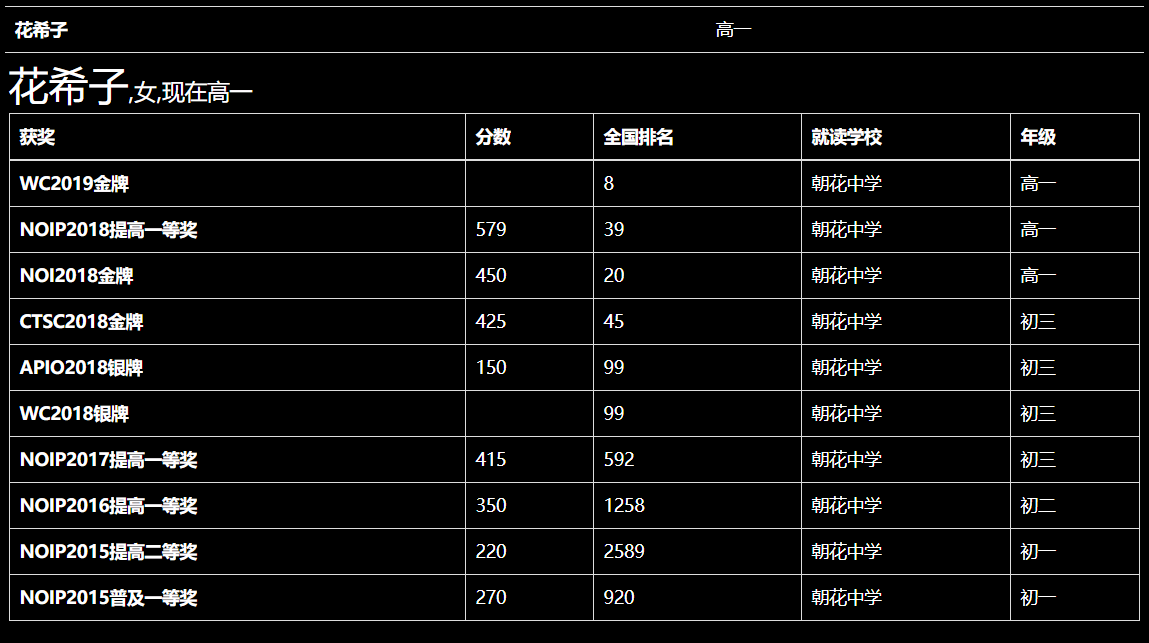
\includegraphics[width=\textwidth]{hanakiko_score.png}
    \end{figure}
\end{frame}
\begin{frame}{致谢与致歉}{致歉}
    事实上,Hanakiko是朝花中学OI队的领头选手。她继承了ugoul的优良传统,OI知识体系完整,\sout{我们}我要多向她学习。\newline 
 
    Hanakiko也如题目中的那样友善可爱,有什么问题也可以咨询她哦,她有问必答(雾)。\newline

    在这里,Sweetlemon为把Hanakiko弱化而道歉。
\end{frame}

\section{T0 泳装}
\begin{frame}{T0 泳装}{历史}
    泳装一题是去年的老题。\\
    去年10月份,我在\href{https://paiza.jp/poh/ando/challenge/f10d2975/ando13}{Piaza Online Hackathon}上看到这道题,便决定把它搬到团队里,谁知无人问津。
    于是,我便把这题作为了这次比赛的公开题。
\end{frame}

\begin{frame}
    \frametitle{T0 泳装}
    \framesubtitle{做法}
    60分:暴力计算出$n!\pmod{10^9}$即可。\newline
    \pause
    如何计算$n!\pmod{10^{9}}$的准确值?
    \begin{itemize}
        \item 使用Python或Java的高精度
        \pause
        \item 使用long long(在小的数据范围内可过)
    \end{itemize}
\end{frame}
\begin{frame}
    \frametitle{T0 泳装}
    \framesubtitle{做法}
    100分:在计算过程中,将含$2$和$5$质因子的部分分开处理,其他部分直接$\mod{10^9}$。\newline
    最后将$2$与$5$的质因子进行消去,剩余的乘到其他部分中就好了。\newline
    \pause
    极其卡常数,一定要注意优化。没有优化好就只有80分了。
\end{frame}
\begin{frame}
    \frametitle{T0 泳装}
    \framesubtitle{做法}
    \temporal<2->{毒瘤Sweetlemon,卡常数!}{\sout{毒瘤Sweetlemon,卡常数!}}{\sout{毒瘤Sweetlemon,卡常数!}}
    \pause
    \newline
    真的没有不需要卡常数的做法么?
\end{frame}
\begin{frame}
    \frametitle{T0 泳装}
    \framesubtitle{做法}
    这不简单!过程中一直$\mod{10^9}$不就好了。\newline
    
    \pause
    然而这是错的。\\
    $50!$的答案是$568960512$,但是这个做法输出的却是$215302144$。\newline

    \pause
    原因是什么呢?
    \pause
    思考这道题与平常模意义下计算的区别。\\
    区别是要去除末尾的$0$。问题就出在这里。\\
    在$k!=(k-1)!\times k$的过程中,可能乘出了一些末尾$0$需要去除,导致之前被模掉的部分重新出现在答案中。\newline

    \pause
    以$\mod{1000}$为例。\\
    $12125\times 4=48500$,上述结果去除末尾$0$后答案应该为$485$,但是如果提前取模,答案就只剩$5$了。
\end{frame}
\begin{frame}
    \frametitle{T0 泳装}
    \framesubtitle{做法}
    于是我们想到,计算过程中多保留几位行不行呢?\\
    \pause
    可是问题又来了,多保留几位后,乘起来就有可能超过long long范围。\\
    这样我们就只能使用龟速乘($\text{O}(\log n)$)或long double快速乘($\text{O}(1)$)。\\
    \pause
    但是很不幸,迎接它们的都是\textcolor{tle}{TLE}!\newline

    \pause
    因此,刚才的问题的答案是:很抱歉,Sweetlemon真的没有发现不需要卡常数的做法。\\
    \pause
    毒瘤Sweetlemon,卡常数!
    
\end{frame}
\begin{frame}
    \frametitle{T0 泳装}
    \framesubtitle{总结}
    这是:
    \begin{itemize}
        \item 一道简单运用性质的数学题
        \item 一道卡常数的毒瘤题
    \end{itemize}
    
\end{frame}

\section{T1 投票}

\begin{frame}{T1 投票}{历史}
    这道题的灵感最早来源于一道逻辑题。
    \begin{block}{逻辑问题}
        在会议上,甲说:“我认为X,Y两人中\textbf{至少}有一人要涨工资。”乙说:“我\textbf{不同意}!”\\
        请问乙的意思是?\\
        \begin{description}
            \item[A] X,Y两人都要涨工资
            \item[B] X,Y两人都不要涨工资
            \item[C] X,Y两人中应恰有一人涨工资
            \item[D] X,Y两人中至多有一人涨工资   
        \end{description}
    \end{block}
    \pause
    个人认为答案是B。“至少一人”即$\ge 1$,其否定是$<1$,即$0$,也即“都不”。

\end{frame}
\begin{frame}{T1 投票}{历史}
    当时这道题是作为动态规划题出的。\\
    \pause
    那么现在它到底还是不是一道动态规划题呢?\\
    \pause
    让我们拭目以待。

\end{frame}

\begin{frame}{T1 投票}{做法}
    \begin{itemize}
        \item 10分:直接枚举唯一的一个议案是否通过即可,是不是很简单?
        \pause
        \item 40分:直接枚举每个议案是否通过即可。$\text{O}(m\times 2^n)$。
        \pause
        \item 70分:动态规划或记忆化搜索。将前两类意见和后两类意见分开考虑。定义状态为“前$i$个议案,通过$j$个,前两类意见的最大收益”,那么很容易写出状态转移方程。最后枚举通过的总议案数即可。$\text{O}(n^2+m)$。
        \pause
        \item 100分:观察我们刚才的状态转移方程,是不是觉得这个方程太简单而且充满了重复?思考一下,在$n$个议案中通过$k$个议案,你会怎么选择?这里就可以用贪心策略。\\
        \pause
        计算出前两类意见中,支持第$i$个议案的总权$a_i$和反对第$i$个方案的总权$b_i$,那么定义议案的“收益”为$a_i-b_i$,显然我们会选择收益最高的$k$个议案。\\
        这样就可以贪心了。将意见按收益排序,然后枚举通过的议案数$k$,累加前$k$大的收益即可。$\text{O}(n\log n+m)$。
    \end{itemize}

\end{frame}
\begin{frame}{T1 投票}{总结}
    这是一道:
    \begin{itemize}
        \item 需要一定思考的贪心题
        \item 垃圾出题人差点搞错做法的题目
    \end{itemize}
\end{frame}
\section{T2 分班}

\begin{frame}{T2 分班}{历史}
    这题不太有历史。\\
    这题是Sweetlemon强行脑补出来的一道题目,主要灵感是二分图匹配算法。\newline

    \pause
    其实这题算是一个模板题。这类问题被称为\textbf{二分图多重匹配}。
\end{frame}
\begin{frame}{T2 分班}{做法}
    \begin{itemize}
        \item 10分:直接输出“1 $\backslash \text{n}$ 1”即可。
        \pause
        \item 20分:将唯一的一个人随意分配到任意一个愿望中的班级即可。
        \pause
        \item 40分:$\text{O}(m^n)$暴力枚举所有方案即可。
        \pause
        \item 50分:60分的数据中包含一个额外的数据点,其中每个人的愿望都只含有一个班级。对于这种情况,只要套用普通的二分图匹配算法即可。
        \pause
        \item 60分:全部算出了正确答案但不输出方案就是60分呀!
        \pause
        \item 分数不定:奇怪的分配方案,如按顺序分配班级。
        \pause
        \item 100分:将匈牙利算法扩展,或使用网络流算法(bushi)。$\text{O(能过)}$。\\其实想到二分图应该就能做出满分算法呀!
    \end{itemize}
\end{frame}
\begin{frame}{T2 分班}{总结}
    这是一道:
    \begin{itemize}
        \item 简单扩展的模板题
        \item \sout{考验网上搜索能力的好题}
    \end{itemize}
\end{frame}

\section{T3 项链}
\begin{frame}{T3 项链}{历史}
    这题是Sweetlemon在听“最小表示法”的时候弄出来的题目,主要是为了介绍这种算法,思维价值不大(Sweetlemon有出过思维价值大的题目么?)
\end{frame}
\begin{frame}{T3 项链}{做法}
    \begin{itemize}
        \item 10分:如果两个字符串长度相同,就输出$1$,否则输出$0$。
        \pause
        \item 30分:暴力匹配两个字符串,匹配成功就输出$1$,否则输出$0$。(有一种技巧叫做倍长串,就是在字符串$s$的后面接上自己,即把$\text{abc}$变成$\text{abcabc}$。这样环串旋转就等价于倍长串的一个子串。)
        \pause
        \item 60分:相当于判断两个环串是否“循环同构”,即其中一个通过旋转能否变成另一个。这也相当于在其中一个串的倍长串中找另一个串的匹配。\\可以用KMP或者Hash(花希$\approx$哈希)$\text{O}(l)$解决。\newline
        
        \pause
        但是这样就没办法得出这道题的正解了呢!当串的数目增多的时候,(似乎)就不能用上面的办法解决问题了。\\
        那么怎么办呢?
    \end{itemize}
\end{frame}
\begin{frame}{T3 项链}{做法}
    我们是怎么判断$39$和$2019$在模$10$的意义下同余呢?\\
    我们计算出了$39$和$2019$除以$10$的余数$9$,即在模$10$的意义下找到了一个“最小代表元素”或“\textbf{最小表示}”,比较这个最小表示是否相同。\\
    同样,并查集的思想也是给在同一个集合里的元素找一个代表元。\newline
    \pause

    概括一下,上面比较两个元素是否同构的办法就是,选择一种表示方法,使得同构的元素表示方法都相同,且不同构的元素表示方法不同。\\
    我们在这里约定,环状字符串的“最小表示”就是通过旋转字符串,能够得到的\textbf{字典序最小}的新串。我们称之为最小表示(或最小表示法)。

\end{frame}
\begin{frame}{T3 项链}{做法}
    这样,这道题目就转化为:求出每个环串的最小表示,计算每个最小表示出现了多少次。\\
    设某个最小表示的出现次数为$x(x>1)$,那么选到这种最小表示的项链的可能情况为$\text{C}^{x}_{2}=\frac{x(x-1)}{2}$。\\
    把所有的上述答案累加起来,除以总可能情况$\text{C}^{n}_{2}=\frac{n(n-1)}{2}$(其实是乘以这个数的逆元),就得到答案了。
\end{frame}
\begin{frame}{T3 项链}{做法}
    如何求出最小表示呢?\newline
    \pause

    先倍长串,然后枚举最小表示在倍长串中的起始位置(简称“位置”),用一个变量存储当前的最小表示位置,不断进行匹配即可。\\
    有一个关键点,就是如果在$k$位置失配,那么枚举指针可以直接跳到$k+1$位置。(我知道我写得很抽象,但是这不是为了赶工么?)\\
    这样可以证明是$\text{O}(n)$的。\\
    详情参考\href{https://blog.csdn.net/tianyuhang123/article/details/54919715}{这篇资料}。(可能我未来也会写一篇博客的吧,咕咕咕。)\newline

    \pause
    求出最小表示之后,就可以用STL的map或者哈希(花希!)求答案了。
\end{frame}
\begin{frame}{T3 项链}{总结}
    这是一道:
    \begin{itemize}
        \item 算法很妙的模板题
        \item 引出一种思想的算法模板
        \item 强行插入组合数学和(简单)数论的题目
    \end{itemize}
    \pause

    我在写样例解释的时候发现了一个问题:题目描述中,概率$\frac{p}{q}$中的$p$和$q$是互质的,但标程中没有保证互质。在紧急修改标程后,我发现,答案\sout{竟然}是一样的!\\
    为什么呢?\sout{证明留作习题。}
\end{frame}
\section{总结与展望}
\begin{frame}{最后的致谢}
    最后,还是要感谢\textcolor{admin}{cultry}的帮助!\\
    感谢各位的积极参与!\\
    感谢\LaTeX 和beamer提供幻灯片制作平台!\\
    欢迎大家期待我的下一场比赛!(咕咕咕……)\newline

    \pause
    我是不是忘了什么?\\
    非常感谢Hanakiko\sout{酱}桑啦!$mua\sim$\\
    \pause
    另外她是我的,你们谁也不许抢(一把带走)
\end{frame}
\end{document}